\section{Implementation and Methodology}
\label{sec:impl}

% 

\begin{table}[!t]
\caption{Datasets used in experiments. We report the number of training/testing samples separately in the column ``All''.}
\label{table-datasets}
\centering
\footnotesize
\begin{tabular}{@{}cccc@{}}
\toprule
\multirow{2}{*}{\textbf{Dataset}} & \multirow{2}{*}{\textbf{\# of Labels}} & \multicolumn{2}{c}{\textbf{\# of Samples}} \\ \cmidrule(l){3-4} 
                         &                              & Per-class     & All              \\ \midrule
Caltech-101~\cite{c101}              & 101                          & 40--800       & 3,060/6,084      \\
Caltech-256~\cite{c256}              & 257                          & 80            & 15,420/15,187    \\
Dogs vs. Cats~\cite{Dvg}            & 2                            & 900           & 1,800/2,000      \\
DTD~\cite{dtd}                      & 47                           & 120           & 3,760/1,880      \\ \bottomrule
\end{tabular}


\end{table}



\begin{table}[!t]
\caption{Details of devices used in the experiments.}
\label{table-hardware}
\centering
\scriptsize
\begin{tabular}{@{}l|l|l@{}}
\toprule
\textbf{Name}                                             & \textbf{Processor}                                                                                                                                   & \textbf{Software env.}                                                                            \\ \midrule
\begin{tabular}[c]{@{}l@{}}Jetson \\ TX2~\cite{tx2}\end{tabular}     & \begin{tabular}[c]{@{}l@{}}Dual-Core NVIDIA Denver 2 64-Bit CPU,\\ 256-core NVIDIA Pascal™ GPU.\end{tabular}                                         & \begin{tabular}[c]{@{}l@{}}Ubuntu 18.04 LTS, \\ PyTorch 1.7.1.\end{tabular}                      \\ \midrule
RPI 4B~\cite{rpi}                                                    & \begin{tabular}[c]{@{}l@{}}Broadcom BCM2711B0 quad-core \\ A72 64-bit @ 1.5GHz CPU.\end{tabular}                                                     & \begin{tabular}[c]{@{}l@{}}Raspbian 11,\\ PyTorch 1.7.1.\end{tabular}                              \\ \midrule
MI 10~\cite{mi10}                                                     & \begin{tabular}[c]{@{}l@{}}2.84GHz Cortex-X1, \\ 3× 2.4GHz Cortex A78, \\ 4× 1.8GHz Cortex A55 CPU.\end{tabular}                                     & \begin{tabular}[c]{@{}l@{}}Android 10, \\ MNN 2.0.0, \\ ONNX 1.13.1.\end{tabular} \\ \cmidrule(r){1-2}
\begin{tabular}[c]{@{}l@{}}Huawei \\ Mate 30~\cite{HuaWei}\end{tabular} & \begin{tabular}[c]{@{}l@{}}2x 2.86 GHz ARM Cortex-A76,\\ 2x 2.09 GHz ARM Cortex-A76,\\ 4x 1.86 GHz ARM Cortex-A55 CPU,\\ Kirin 990 NPU.\end{tabular} & \begin{tabular}[c]{@{}l@{}}Android 10, \\ MNN 2.0.0, \\ ONNX 1.13.1.\end{tabular} \\ \bottomrule
\end{tabular}



\end{table}

\begin{figure*}[!t]
  
    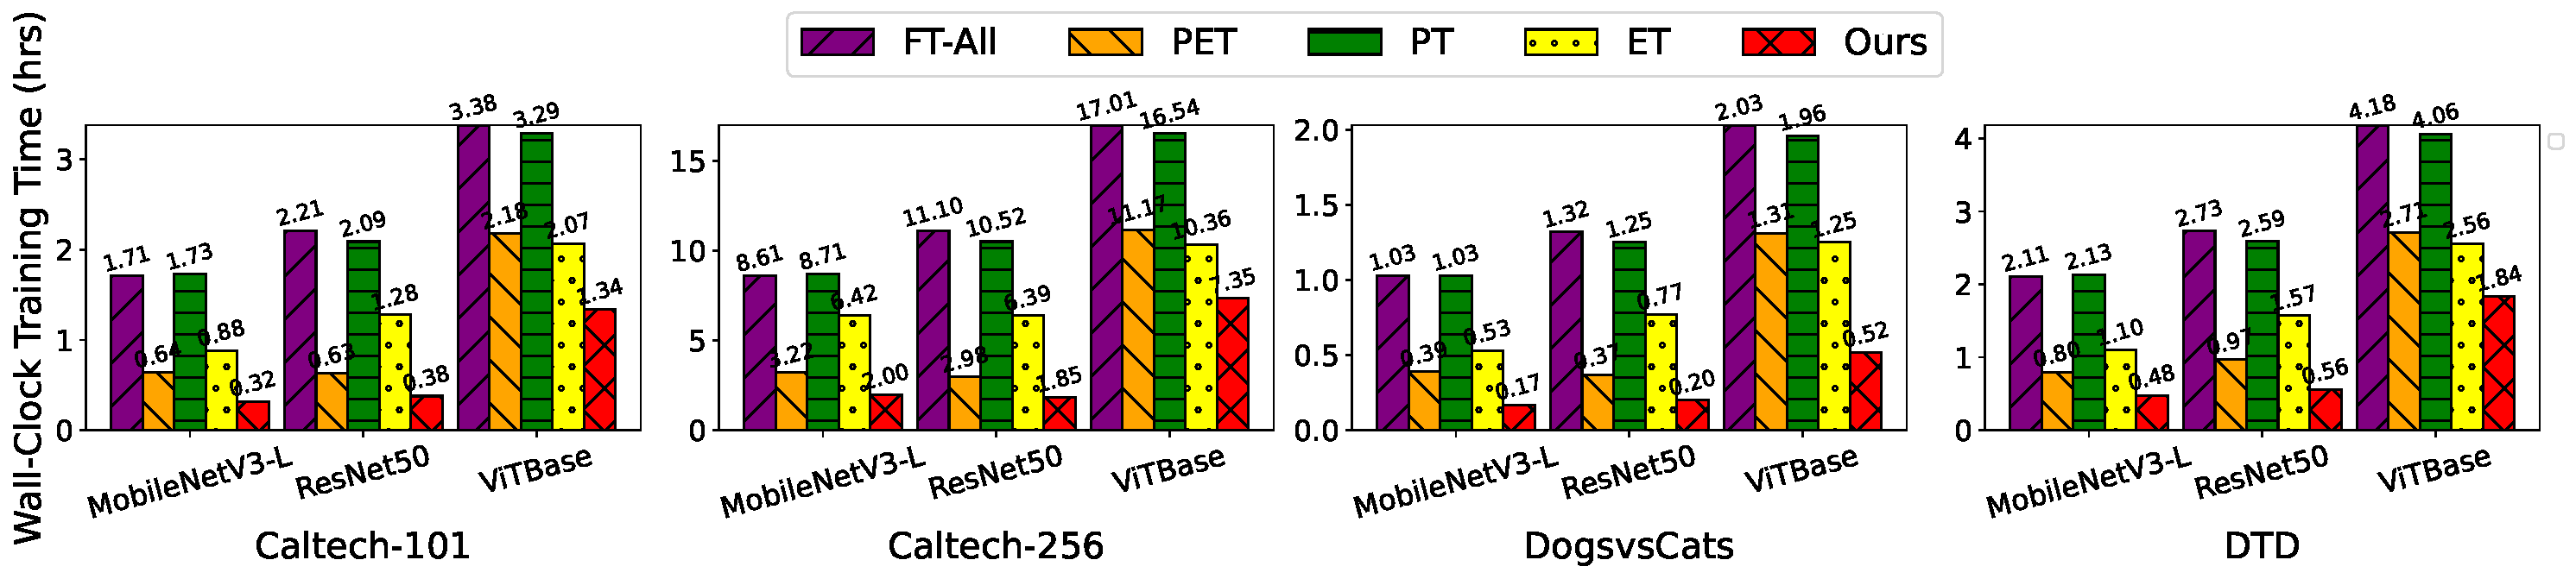
\includegraphics[width=0.97\textwidth]{figs/wallclocktime.pdf}

  \caption{Wall-clock on-device training time. Device: Jetson TX2.}
  
  \label{fig:e2etime}
\end{figure*}




\noindent \textbf{System implementation.}
We have fully implemented a \sys prototype with 4k LoC in Python and 3k LoC in C/C++ atop PyTorch and MNN~\cite{MNN}.
All the techniques of \sys can work in other ML frameworks designed for different devices and runtime environments like TensorFlow~\cite{tf} and TFLite~\cite{tflite}.
At the cloud side, we use a GPU server with 4× NVIDIA A40. 
At the edge side, we use devices described in Table ~\ref{table-hardware}.

% Both the NVIDIA Jetson TX2 and the Raspberry Pi 4B are widely used develop board on embedded platforms such as drones, smart cars and robots.
% Jetson TX2 is equipped with a Nvidia Pascal GPU with 256 CUDA cores, a 1.2GHz Cortex-A57 CPU and 8GB memory shared between GPU and CPU; Raspberry Pi 4B is equipped with a 1.5GHz Cortex-A72 CPU and 4GB memory.
% We also evaluate our system on a off-the-shelf smartphone MI10 which is equipped with a Snapdragon 865 SoC, and the experiments are run on CPU with 4 big cores.
% For Jetson TX2 and Raspberry Pi 4B, we use the Ubuntu 18.04 LTS OS with PyTorch 1.12.1;
% for MI10, we use the Android OS 10 with MNN 2.0.0 and ONNX 1.13.1.
% There are also several third-party libraries used at cloud pre-training stage, e.g., Once-For-All~\cite{} and Torch-Pruning~\cite{} for structural pruning and Pytorch Profiler~\cite{} and THOP~\cite{} for latency table profiling. 

\noindent \textbf{Models, datasets and metrics.}
% \mwx{have a table for models and datasets}
We evaluate \sys with the following representative models: MobileNetV3-L~\cite{howard2019searching}, ResNet50~\cite{he2015deep} and ViT\_base~\cite{dosovitskiy2021an}.
% These models encompass various architectures, computational costs, and capacities, and are specified with different trainable components during on-device fine-tuning.
% For MobileNetV3, we fine-tune only the head; for ResNet50, we fine-tune the head and an adapter; for VIT base, we fine-tune the head and 6 adapters. 
% All the adapters used in each model have the same latent size and are inserted layer by layer starting from the model’s output layer moving forward.
We on-cloud pre-train these models with the ImageNet2012~\cite{ImageNet2012} dataset that contains 1.2M images, and then on-device fine-tune them with the downstream datasets (Caltech-101~\cite{c101}, Caltech-256~\cite{c256}, Dogs vs. Cats~\cite{Dvg}, DTD~\cite{dtd}) which are more fine-grained.
We mainly focus on the following metrics: \textit{the wall-clock on-device training time} and \textit{the best test accuracy}.
% \begin{itemize}[leftmargin=*]
% \item \textbf{Caltech-101} with 3,060 training data and 6,084 testing data. 
% It contains 101 long-tailed distributed categories of images, with approximately 40 to 800 images per category, including common objects such as animals and vehicles.    

% \item \textbf{Caltech-256} with 15,420 training data and 15,187 testing data, which is 
% an extended version of Caltech-101, with more complicated classification categories and similarly fewer samples per category (80 in average).

% \item \textbf{Dogs vs. Cats} with 25,000 images of dogs and cats.
% It is relatively simple but serves as a very classic benchmark dataset for evaluating transfer learning performance in downstream tasks.
% We sample a subset of 1,800 training data and 2,000 testing data from the parent dataset, with an equal number of cats and dogs.

% \item \textbf{DTD} with 3,760 training data and 1,880 testing data.
% Unlike the previous datasets, the DTD (Describable Textures Dataset) contains 47 different categories of texture images. 
% These texture categories include various materials, object surfaces, and natural textures such as grass, bark, water, fabric, brick walls, and more. 
% Each texture category consists of approximately 120 images.
% \end{itemize}



\begin{table*}[!t]
\caption{Accuracy of \sys and baselines. C-101: Caltech-101; C-256: Caltech-256; DVC: Dogs vs. Cats.}
\label{table-e2e accuracy}
\centering

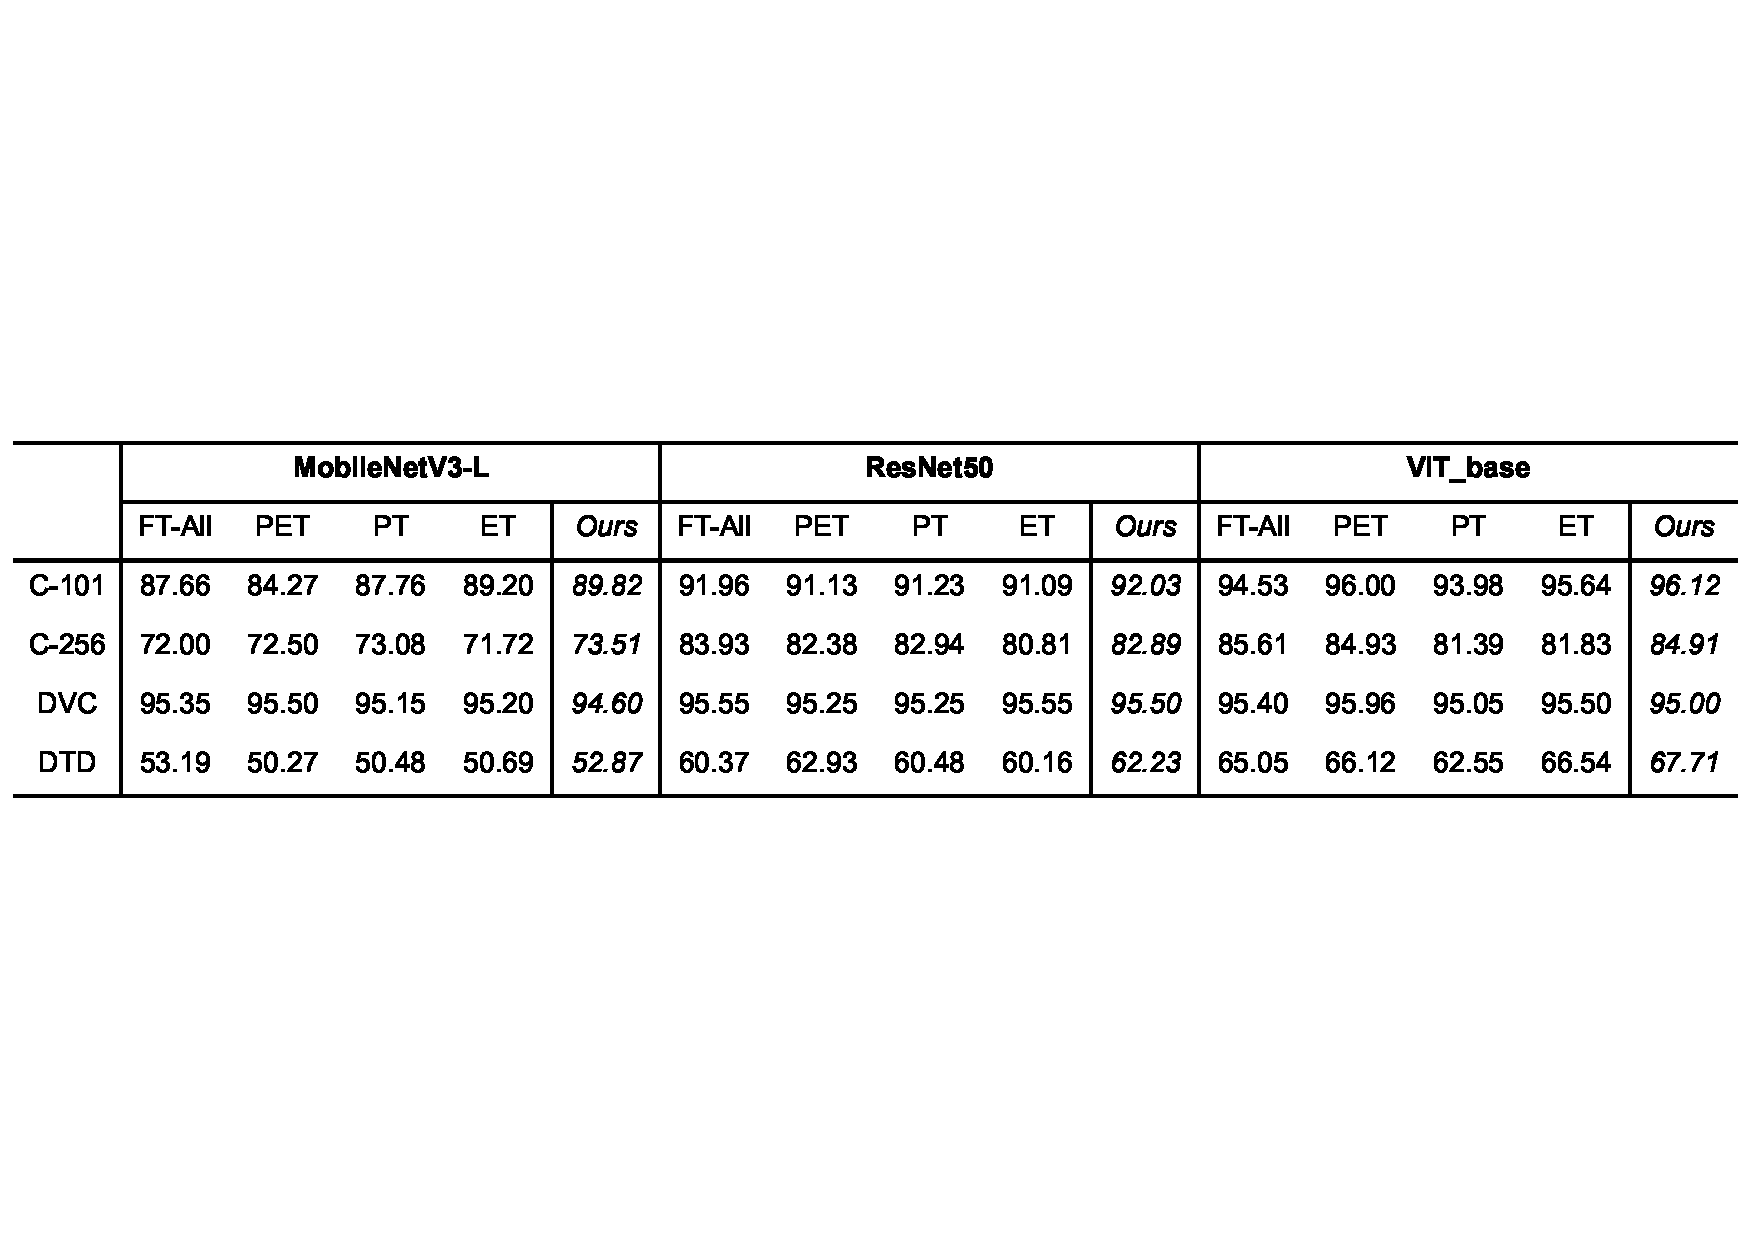
\includegraphics[width=0.80\textwidth]{figs/dynaproxyer_acc.pdf}




\end{table*}


\noindent \textbf{Baselines.}
We compare \sys to these alternatives:
% \begin{itemize}[leftmargin=10pt, topsep=0pt]
Fine-tuning all parameters (\texttt{FT-All}) always fine-tunes the whole pre-trained NN. This is the default fine-tuning methodology used in most pre-training-and-fine-tuning paradigms.
Parameter-Efficient Training (\texttt{PET}) freezes most layers of the pre-trained NN and trains only a small portion. We evaluate various PET methods: Linear Probing~\cite{kumar2022finetuning} for ResNet50, Last-3~\cite{guo2019spottune, MLSYS2019_e09d45e1} for MobileNetV3 and Adapters(12)~\cite{rebuffi2017learning, houlsby2019parameter} for ViT\_base.
PruneTrain (\texttt{PT})~\cite{10.1145/3295500.3356156} is a framework that dynamically prunes the NN during training. %It profiles the importance of channels at runtime and gradually removes less important channels to reduce the end-to-end training time.
ElasticTrainer (\texttt{ET})~\cite{huang2023elastictrainer} is one of the state-of-the-art on-device training frameworks that dynamically determines trainable layers by estimating the importance of NN tensors.

\noindent \textbf{Hyper-parameters.}
% We empirically use the following hyper-parameters:
The momentum coefficient $m$ of PruneTrain is 0.8.
% The pruning step $d$ is 10\%. 
% The number of proxy networks is 10.
The L1 penalty coefficient of PruneTrain is set to 1e-4.
The ratio $\rho$ of ElasticTrainer is set to 0.4.
To provide big-enough search space, we on-cloud generate $N=10$ proxy sub-networks with a pruning step size $d=7\%$--$10\%$. 
Limited by the memory constraint of edge devices, the mini-batch size is set to 4.
Training epochs are set to 12 following prior work ~\cite{huang2023elastictrainer}.
% The learning rate is 1e-4. 
% The optimizer is standard SGD.
Training samples are resized to a 224$\times$224 RGB image with standard data augmentation strategies such as random cropping and flipping.



\begin{figure}[!t]
	\centering
	\subfloat[Time to accuracy\label{fig:time2acc}]{%
  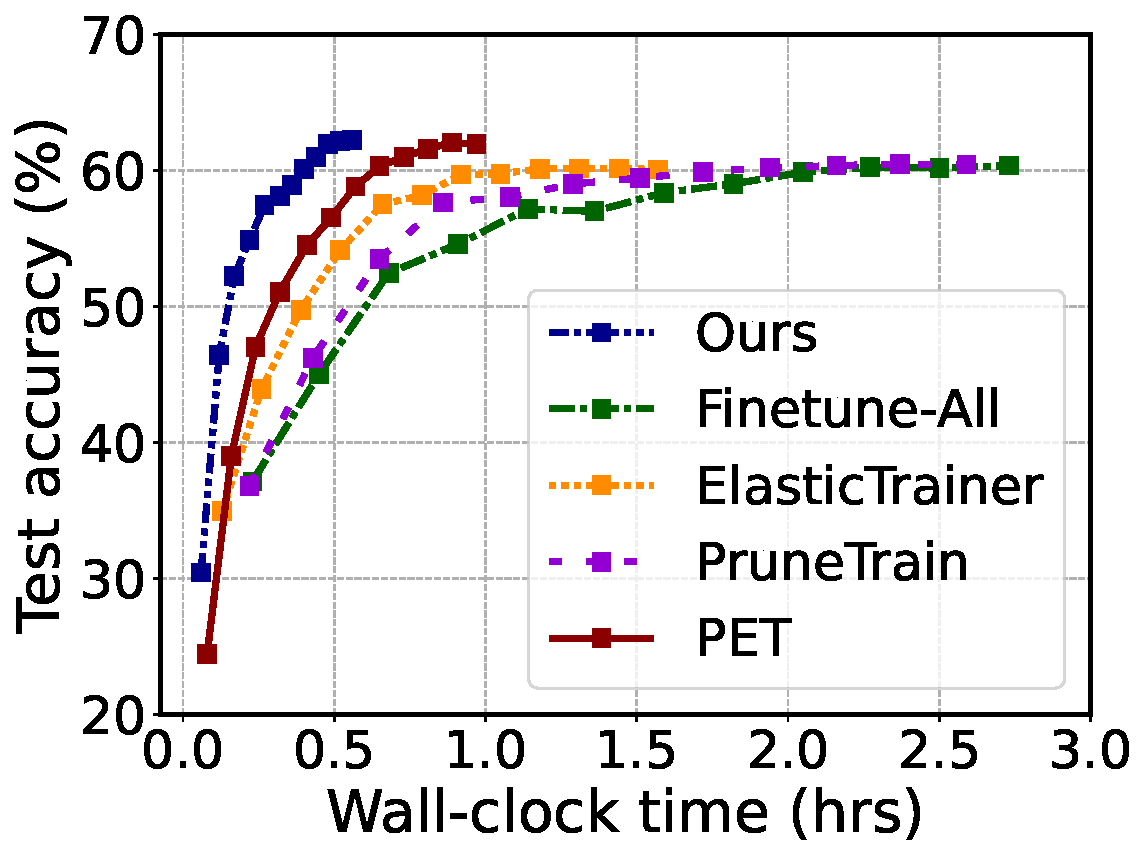
\includegraphics[width=0.55\linewidth]{figs/time2acc.pdf}}
        \hfill
	\subfloat[Speedup\label{fig:speedup2acc}]{%
  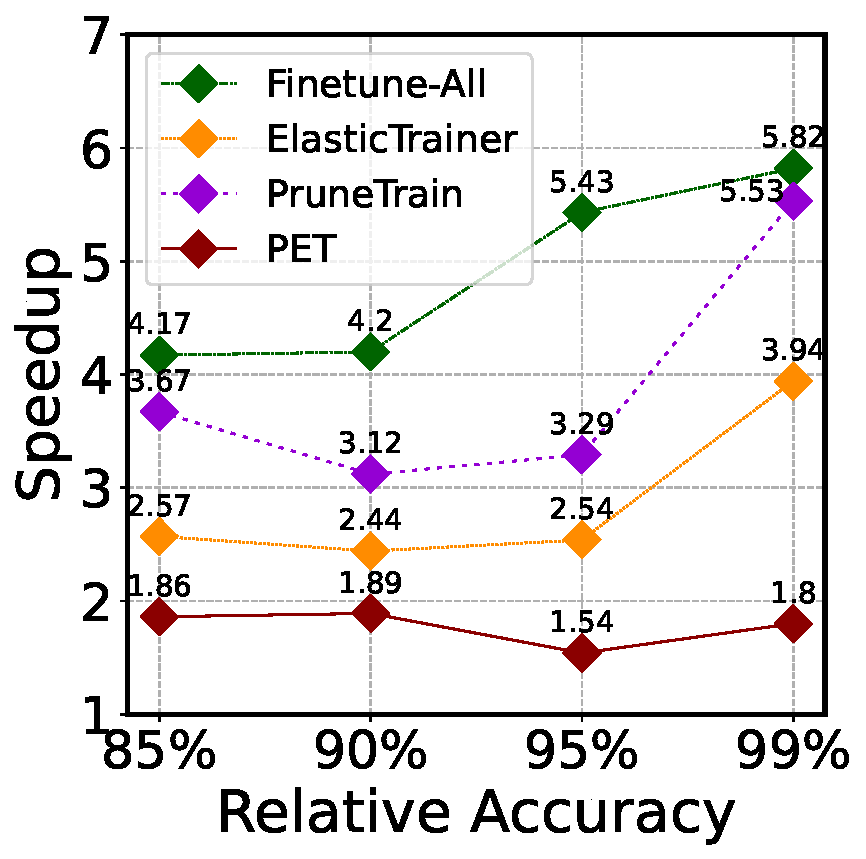
\includegraphics[width=0.43\linewidth]{figs/speedup2acc.pdf}}
        
	\caption{\sys achieves significant speedup across different accuracy targets. Model: ResNet50; Dataset: DTD.}
        
        \label{targeted acc}
\end{figure}
